\chapter{Smart Pointers}

In our journey through Rust, we have seen how the ownership model, combined with borrowing rules, ensures memory safety without a garbage collector. However, these strict compile-time rules can sometimes feel restrictive. What if you need to build a complex data structure like a graph, where a single node might be pointed to by multiple edges? What if you want to extend the lifetime of a variable created inside a function so that it outlives the function call, without losing the ability to clean it up automatically?

To solve these problems, Rust relies on \textit{smart pointers}. The concept of a smart pointer is not unique to Rust; it was born much earlier in the C++ ecosystem (with \texttt{unique\_ptr}, \texttt{shared\_ptr}, and \texttt{weak\_ptr}) and was subsequently adopted and expanded upon by Rust. In Rust, smart pointers are data structures that act like pointers but encapsulate additional metadata and powerful guarantees. 

\begin{insightbox}
\textbf{The Magic of Traits and Operator Overloading} \\
In C++, the concept of smart pointers relies heavily on operator overloading---extending the meaning of operators like \texttt{*} or \texttt{->} for custom types. Rust adopts a similar philosophy using traits. Under the hood, all smart pointers in Rust are just structs that implement two crucial traits:
\begin{itemize}
    \item \texttt{Deref} (and \texttt{DerefMut}): Allows the smart pointer to behave like a standard reference, enabling you to use the \texttt{*} operator to access the underlying data seamlessly. This lets the compiler automatically perform deref coercions.
    \item \texttt{Drop}: Dictates what happens when the smart pointer goes out of scope, typically handling the automatic deallocation of the heap memory.
\end{itemize}
\end{insightbox}

% --- Section: Box ---
\section{Exclusive Ownership on the Heap: \texttt{Box<T>}}

The simplest and most common smart pointer is \texttt{Box<T>}. A \texttt{Box} allows you to store data on the heap rather than the stack. The box itself---which is essentially just a pointer---remains on the stack, while the data it points to lives on the heap.

\subsection*{Usage Guidelines: When and Why to Use \texttt{Box<T>}}
\begin{itemize}
    \item \textbf{When you have a type whose size can't be known at compile time} and you want to use it in a context that requires an exact size (e.g., recursive types, trait objects).
    \item \textbf{When you have a large amount of data} and you want to transfer ownership without copying the data byte-by-byte across the stack.
\end{itemize}

\subsection*{Building Intuition: Why use a Box?}
Consider a function that creates a piece of data. Normally, local variables live on the stack and vanish as soon as the function returns. If we want the caller to own this data without copying potentially large structures byte-by-byte across the stack, we can allocate it on the heap. 

\begin{lstlisting}[language=Rust]
fn produce(modify: bool) -> Box<i32> {
    let mut b = Box::new(0); // Allocates memory on the heap
    
    if modify {
        *b = 5; // Dereferencing allows us to modify the heap data
    }
    
    b // The box is returned, transferring ownership to the caller
}

fn main() {
    let b1 = produce(false);
    let b2 = produce(true);
} // b1 and b2 are dropped here, and their heap memory is safely freed
\end{lstlisting}

\textbf{Deep Memory Model Analysis:} When \texttt{produce} is called, the stack frame holds the \texttt{modify} parameter and the local variable \texttt{b}. \texttt{Box::new(0)} allocates exactly 4 bytes (for an \texttt{i32}) on the heap, and \texttt{b} stores the 8-byte pointer to this heap allocation. If \texttt{modify} is true, the heap data is mutated in place via dereferencing (\texttt{*b = 5}). Returning \texttt{b} transfers ownership: the 8-byte pointer is moved from \texttt{produce}'s stack frame to \texttt{main}'s stack frame (into \texttt{b1} or \texttt{b2}). The heap allocation itself remains untouched during this move. Finally, when \texttt{b1} and \texttt{b2} go out of scope at the end of \texttt{main}, their lifetimes end, triggering the \texttt{Drop} trait which deallocates the corresponding heap memory exactly once, avoiding any memory leak or double-free vulnerabilities.

\begin{examprioritybox}
\textbf{Professor's Emphasis: Avoiding Leaks and Double Freeing} \\
In C and C++, allocating memory with \texttt{malloc} requires explicitly calling \texttt{free}. Forgetting to do so causes a memory leak, while calling \texttt{free} twice causes undefined behavior. By tying the heap allocation to the lifetime of the \texttt{Box}, Rust completely eliminates both vulnerabilities.

\textbf{Common Pitfall:} Assuming moving a \texttt{Box} copies the heap data. It only moves the pointer on the stack, transferring exclusive ownership without copying the underlying heap data.
\textbf{Expected Mastery Level:} Very High. You must thoroughly understand how the \texttt{Drop} trait is tied to the \texttt{Box}'s scope to guarantee exactly-once deallocation.
\end{examprioritybox}

\subsection*{Fat Pointers vs. Thin Pointers}
If the compiler knows the size of the data stored in a \texttt{Box} (e.g., \texttt{Box<i32>}), the pointer is simply an 8-byte memory address on a 64-bit architecture. This is called a \textit{thin pointer}.

However, boxes are incredibly useful for storing \textit{unsized types} (types whose size is not known at compile time), such as slices (\texttt{[T]}) or trait objects (\texttt{dyn Trait}). When a \texttt{Box} points to an unsized type, it becomes a \textit{fat pointer} (taking up 16 bytes on a 64-bit architecture). 
\begin{itemize}
    \item \textbf{Slices (\texttt{Box<[T]>}):} The first 8 bytes point to the heap data, and the second 8 bytes store the length of the slice.
    \item \textbf{Trait Objects (\texttt{Box<dyn Debug>}):} The first 8 bytes point to the heap data, and the second 8 bytes point to a vtable used for dynamic dispatch. As the professor details, the vtable contains a sequence of entries: the first is the pointer to the drop logic, the second is the size of the concrete type, the third is its alignment, and the subsequent entries are the methods offered by the trait (e.g., the formatting method for \texttt{Debug}).
\end{itemize}

\begin{figure}[H]
    \centering
    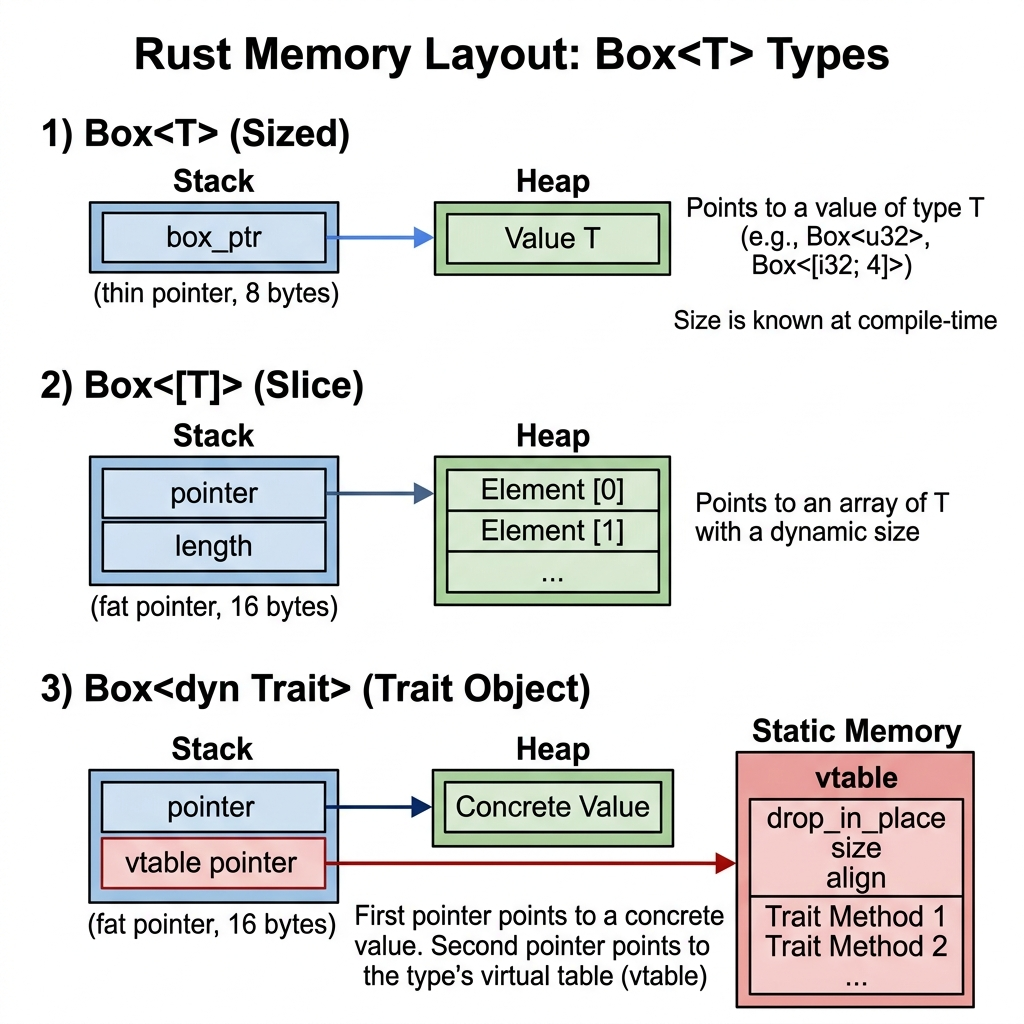
\includegraphics[width=0.85\textwidth]{images/box_memory_layouts.png}
    \caption{The three fundamental memory layouts of \texttt{Box<T>}: A thin pointer for sized types, a fat pointer with length for slices, and a fat pointer with a vtable for trait objects.}
    \label{fig:box_memory}
\end{figure}

% --- Section: Rc ---
\section{Shared Ownership: \texttt{Rc<T>} and \texttt{Arc<T>}}

While \texttt{Box<T>} works flawlessly for exclusive ownership, there are scenarios where a single piece of data must be owned by multiple parts of your program. Consider a Directed Acyclic Graph (DAG) or a complex tree where multiple child nodes need to reference the same parent. 

This brings us to the \texttt{Rc<T>} (Reference Counted) smart pointer.

\subsection*{Usage Guidelines: When and Why to Use \texttt{Rc<T>}}
\begin{itemize}
    \item \textbf{When multiple parts of your program need to read the same data} concurrently in a single-threaded context.
    \item \textbf{When you cannot determine at compile time} which part of the program will finish using the data last.
\end{itemize}

\subsection*{How Reference Counting Works}
\texttt{Rc<T>} keeps track of the number of active references to a value. When you create an \texttt{Rc}, its internal counter is initialized to 1. Every time you duplicate the pointer using \texttt{Rc::clone}, the counter increments. Crucially, this does \textit{not} clone the underlying data; it merely copies the pointer and increases the reference count. 

When an \texttt{Rc} goes out of scope, the counter decrements. The actual heap memory is only freed when the counter hits zero, meaning there are no more active owners.

\begin{insightbox}
\textbf{Reference Counting vs. Garbage Collection} \\
Languages like Java or Python use a Garbage Collector (typically a "Mark-and-Sweep" algorithm) to manage memory. A Mark-and-Sweep GC periodically traverses the entire heap from the root variables to find active allocations, cleaning up unreferenced ones. However, this process often requires pausing the entire program (a "stop-the-world" event), making it unsuitable for real-time applications. Rust's \texttt{Rc<T>} provides a deterministic alternative: memory is freed the exact moment the last reference disappears, without global pauses, at the cost of requiring the programmer to explicitly handle reference cycles.
\end{insightbox}

\begin{lstlisting}[language=Rust]
use std::rc::Rc;

enum List {
    Cons(i32, Rc<List>),
    Nil,
}

use List::{Cons, Nil};

fn main() {
    // We create an Rc pointing to our base list: 5 -> 10 -> Nil
    let a = Rc::new(Cons(5, Rc::new(Cons(10, Rc::new(Nil)))));
    
    // Both 'b' and 'c' can now share ownership of list 'a'
    let b = Cons(3, Rc::clone(&a)); // Reference count of 'a' becomes 2
    let c = Cons(4, Rc::clone(&a)); // Reference count of 'a' becomes 3
}
\end{lstlisting}

\textbf{Deep Memory Model Analysis:} When \texttt{a} is created, the list nodes are allocated on the heap. The variable \texttt{a} on the stack holds an 8-byte pointer to the \texttt{Cons(5, ...)} heap block, which internally contains a \texttt{strong\_count} (initialized to 1). When \texttt{Rc::clone(\&a)} is called for \texttt{b} and \texttt{c}, no new heap allocations for the shared list elements are created. Instead, the \texttt{strong\_count} in the heap is incremented to 2, then 3. \texttt{b} and \texttt{c} are allocated on the stack with their own list head, but their \texttt{Rc} fields point to the exact same heap address as \texttt{a}. When \texttt{c}, \texttt{b}, and \texttt{a} go out of scope, the \texttt{strong\_count} is decremented. Only when it reaches 0 (after the last owner drops) does the heap block invoke its drop logic, cascading the deallocation down the chain.

\begin{warningbox}
\textbf{Calling Associated Functions on \texttt{Rc}} \\
When interacting with the reference counter itself (e.g., checking the count), use the fully qualified syntax \texttt{Rc::strong\_count(\&a)} rather than \texttt{a.strong\_count()}. This prevents naming collisions if the underlying data \texttt{T} happens to have a method named \texttt{strong\_count}. Because \texttt{strong\_count} is an associated function and not a method taking \texttt{self}, the compiler avoids ambiguity. The variable \texttt{a} behaves seamlessly as the inner type for method calls, while \texttt{Rc}-specific operations require explicit functional notation.
\end{warningbox}

\subsection*{The Cost of Synchronization: \texttt{Rc} vs \texttt{Arc}}
You might wonder: is \texttt{Rc} safe to use across multiple threads? The answer is \textbf{no}. The increments and decrements to the reference counter are standard, non-atomic operations. In a multithreaded context, race conditions could cause the counter to become corrupted, leading to double-frees or memory leaks.

\begin{insightbox}
\textbf{Professor's Insight: Unprotected Increments} \\
If you were to write a similar unprotected reference counter in C and modify it concurrently across multiple threads, the results would be disastrous. You would observe the counter increasing randomly, missing increments entirely, or even sporadically going backward due to race conditions. This is undefined behavior at its finest. Rust prevents this entirely by disallowing \texttt{Rc} to be sent across threads.
\end{insightbox}

\begin{figure}[H]
    \centering
    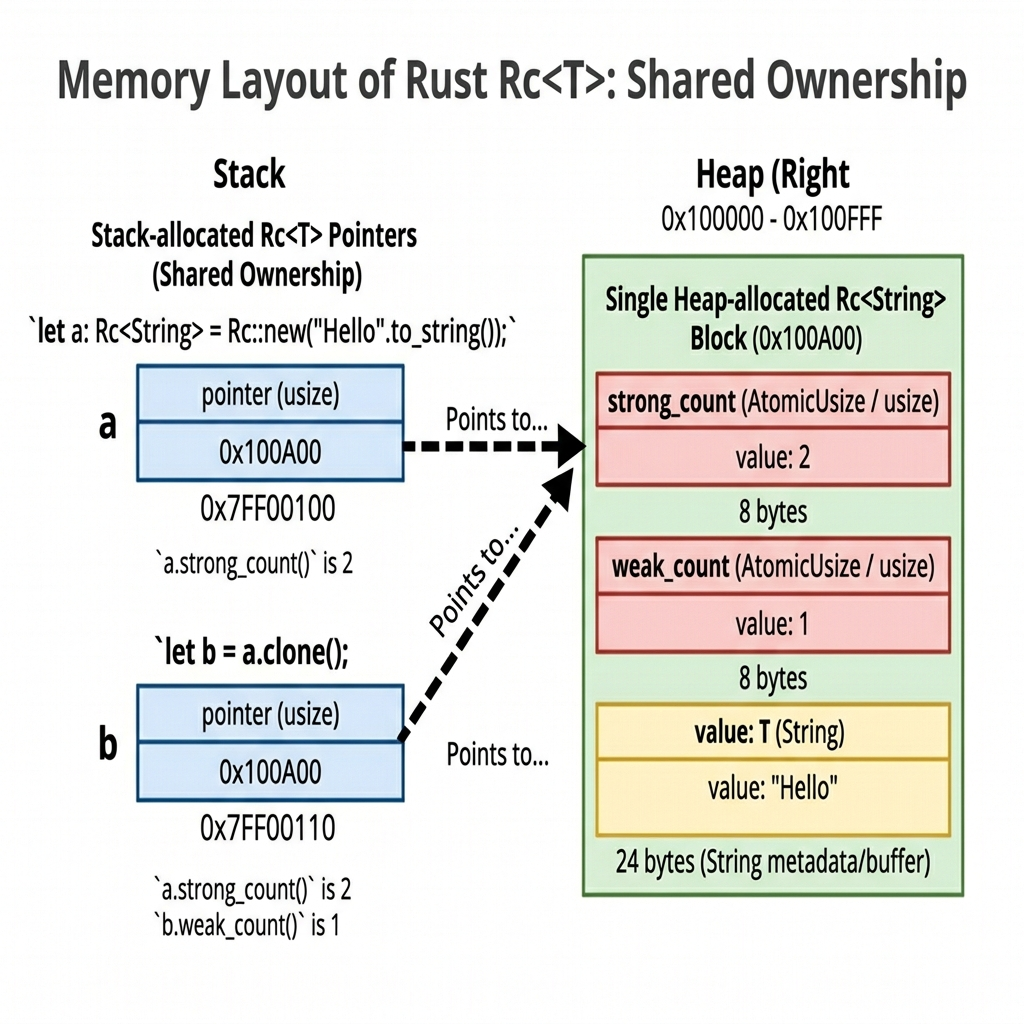
\includegraphics[width=0.85\textwidth]{images/rc_memory_layout2.png}
    \caption{Under the hood: Memory layout of \texttt{Rc<T>}. The heap block contains a strong count, a weak count, and the actual value. Multiple stack pointers share ownership of this single heap block.}
    \label{fig:rc_arc}
\end{figure}

To solve this, Rust provides \texttt{Arc<T>} (Atomic Reference Counted). \texttt{Arc} uses atomic CPU instructions to update the counter, guaranteeing thread safety. However, atomic operations are slightly slower than normal arithmetic. In true Rust fashion (zero-cost abstractions), the language does not force you to pay for thread safety if you don't need it. 
\begin{itemize}
    \item Use \textbf{\texttt{Rc<T>}} in single-threaded contexts.
    \item Use \textbf{\texttt{Arc<T>}} in concurrent contexts.
\end{itemize}

\begin{examprioritybox}
\textbf{Professor's Emphasis: The Cost of Synchronization (\texttt{Rc} vs \texttt{Arc})} \\
Unlike C++ which only provides the thread-safe \texttt{shared\_ptr} (forcing you to pay synchronization costs even in single-threaded contexts), Rust gives you a choice. Use \texttt{Rc} for fast, non-atomic reference counting in single-threaded programs, and \texttt{Arc} for safe, atomic reference counting in concurrent ones.

\textbf{Common Pitfall:} Believing \texttt{Rc} is thread-safe or trying to pass it across threads. The compiler will catch this because \texttt{Rc} does not implement the \texttt{Send} trait, but you must know \textit{why} (non-atomic counter updates lead to race conditions and memory corruption).
\textbf{Expected Mastery Level:} High. Be prepared to justify the choice between \texttt{Rc} and \texttt{Arc} based on concurrency needs.
\end{examprioritybox}

% --- Section: Mutating Shared Data ---
\section{Safely Mutating Shared Data}

By default, an \texttt{Rc} (or \texttt{Arc}) provides \textit{immutable} shared access. If multiple variables point to the same value, modifying it underneath them would violate Rust's core rule: you cannot have mutable and immutable aliases active simultaneously. 

So, how can we mutate data hidden inside an \texttt{Rc}?

\subsection*{Copy-on-Write: \texttt{Rc::make\_mut} and \texttt{Rc::get\_mut}}
If you can prove that you are the \textit{only} owner of an \texttt{Rc} at a given time, you are allowed to mutate it. \texttt{Rc::get\_mut} checks if the reference count is exactly 1 and returns an \texttt{Option<\&mut T>}.

If the count is greater than 1, you can use \texttt{Rc::make\_mut}. This function performs a \textit{Copy-on-Write} (CoW): it clones the underlying data into a new heap allocation, decrements the old counter, and points your \texttt{Rc} to the new, uniquely owned copy.

\begin{lstlisting}[language=Rust]
use std::rc::Rc;

// --- get_mut example ---
let mut a = Rc::new(String::from("abc"));
// Since 'a' is the unique owner (strong_count == 1), get_mut succeeds.
if let Some(s) = Rc::get_mut(&mut a) {
    s.push('!'); 
}
// 'a' now contains "abc!"

// --- make_mut example ---
let mut x = Rc::new(String::from("hello"));
let y = Rc::clone(&x); // Count is now 2

// x and y point to the same string.
Rc::make_mut(&mut x).push('!');

// Now x is "hello!" and y is "hello". 
// make_mut cloned the data because the count was > 1.
\end{lstlisting}

\textbf{Deep Memory Model Analysis:} 
In the \texttt{get\_mut} example, \texttt{a} is the sole owner. \texttt{Rc::get\_mut} safely returns a mutable reference (\texttt{Option<\&mut String>}), allowing direct in-place mutation without any new allocations. If a second reference existed, \texttt{get\_mut} would return \texttt{None} to prevent mutating data shared with others.

In the \texttt{make\_mut} example, initially, both \texttt{x} and \texttt{y} on the stack point to the same heap allocation containing the string \texttt{"hello"}, with a \texttt{strong\_count} of 2. When \texttt{Rc::make\_mut(\&mut x)} is called, the system detects \texttt{strong\_count > 1}. It performs a new heap allocation to clone the string, decrements the \texttt{strong\_count} of the original allocation (so \texttt{y}'s target now has a count of 1), and updates \texttt{x}'s pointer to point to the new, uniquely owned heap block (count of 1). The \texttt{push('!')} operation then mutates only \texttt{x}'s new heap allocation. \texttt{y} remains completely unaffected, preserving memory safety and the immutability guarantee for shared aliases.

\subsection*{Internal Mutability: \texttt{Cell} and \texttt{RefCell}}
What if you absolutely must mutate the shared data \textit{without} copying it? This is where the concept of \textbf{Internal Mutability} comes in. Rust provides types like \texttt{Cell<T>} and \texttt{RefCell<T>}, which allow you to mutate their inner data even if the cell itself is accessed via an immutable reference. These types are meant for single-threaded contexts.

\textbf{Usage Guidelines: When and Why to Use \texttt{Cell} and \texttt{RefCell}}
\begin{itemize}
    \item \textbf{When you need to mutate data} but only have an immutable reference to it (e.g., mutating a field within an \texttt{Rc}).
    \item \textbf{\texttt{Cell<T>}} is preferred for simple types that implement \texttt{Copy} (like integers), as it moves/copies values.
    \item \textbf{\texttt{RefCell<T>}} is preferred for complex types where you need references, moving borrow checking to runtime.
\end{itemize}

\begin{itemize}
    \item \textbf{\texttt{Cell<T>}}: Achieves internal mutability by copying or moving values in and out of the cell. It does not return references to the inner data. Instead, it offers methods like \texttt{set()}, \texttt{get()} (if \texttt{T} implements \texttt{Copy}), \texttt{replace()}, and \texttt{take()} to swap the contents.
    \item \textbf{\texttt{RefCell<T>}}: Allows you to obtain references to the inner data (\texttt{Ref} and \texttt{RefMut}) using the \texttt{borrow()} and \texttt{borrow\_mut()} methods. By wrapping your data in a \texttt{RefCell} inside an \texttt{Rc} (i.e., \texttt{Rc<RefCell<T>>}), you achieve a powerful pattern: shared, mutable ownership. The catch? The borrowing rules are shifted from \textit{compile-time} to \textit{runtime}. If you try to acquire two mutable references to the data at the same time using a \texttt{RefCell}, your program will panic and crash instead of giving a compilation error.
\end{itemize}

\begin{figure}[H]
    \centering
    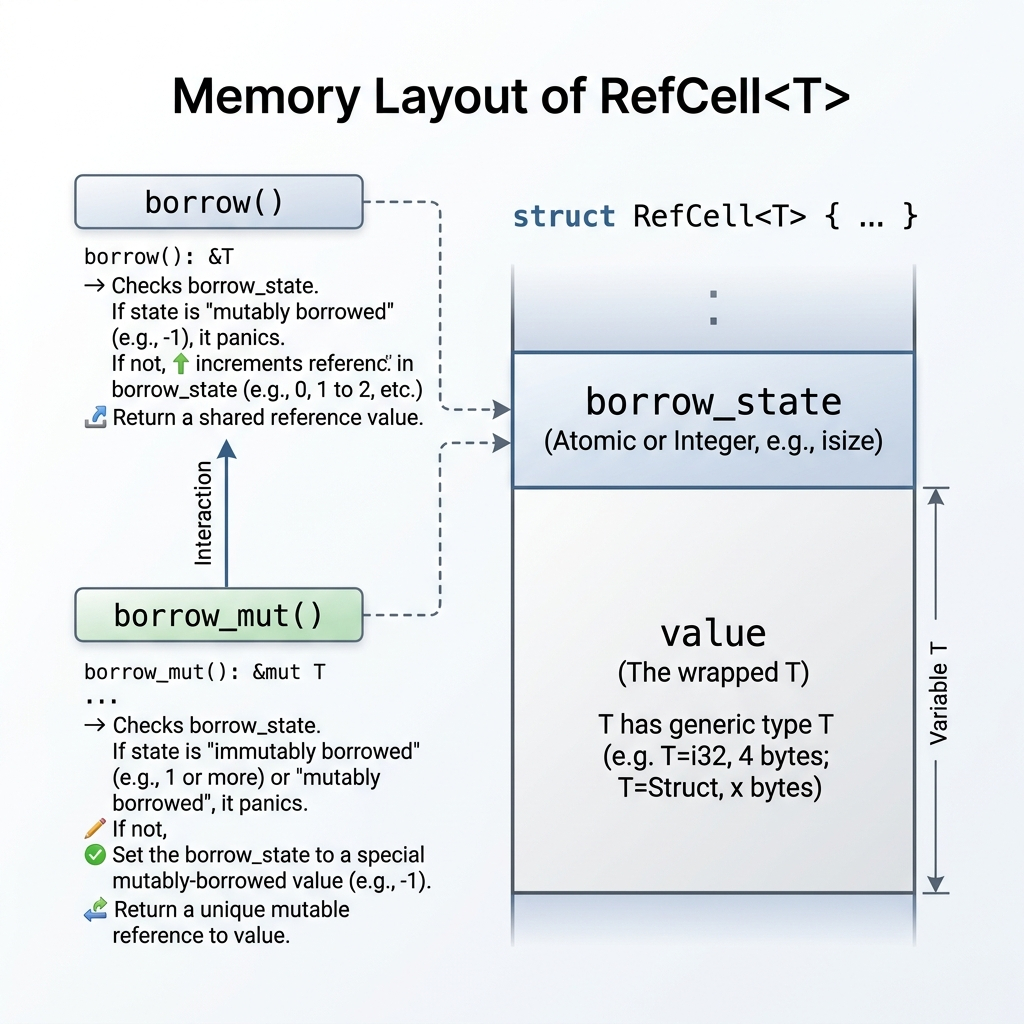
\includegraphics[width=0.7\textwidth]{images/refcell_memory_layout.png}
    \caption{Under the hood: Memory layout of a \texttt{RefCell<T>}. It wraps the inner value alongside a \texttt{borrow\_state} counter to dynamically enforce Rust's borrowing rules at runtime.}
    \label{fig:refcell_memory}
\end{figure}
\subsection*{Clone-on-Write: \texttt{Cow<'a, B>}}
Rust offers another unique smart pointer: \texttt{std::borrow::Cow} (Clone-on-Write). It is an enum that can hold either a borrowed reference (\texttt{Borrowed}) or an owned value (\texttt{Owned}). 

\texttt{Cow} is extremely useful when you want to read data without copying it, but you might occasionally need to mutate it. If you try to mutate a \texttt{Borrowed} variant, \texttt{Cow} will lazily clone the data, become an \texttt{Owned} variant, and apply the mutation, leaving the original data untouched. If the data is already \texttt{Owned}, it modifies it in place without extra allocations. This pattern drastically reduces unnecessary heap allocations when modifications are rare.

% --- Section: Breaking Cycles ---
\section{Breaking Cycles with \texttt{Weak<T>}}

Reference counting has one fundamental flaw: memory leaks caused by \textbf{reference cycles}. 
Imagine object A has an \texttt{Rc} pointing to object B, and object B has an \texttt{Rc} pointing back to object A. Both reference counts are at least 1. Even if all external variables pointing to A and B are dropped, their internal pointers keep each other's counts at 1. The memory will never be freed.

To fix this, Rust provides \texttt{Weak<T>}. 
While cloning an \texttt{Rc} increments the \textit{strong} counter, downgrading an \texttt{Rc} to a \texttt{Weak} pointer increments the \textit{weak} counter. 
Crucially, \textbf{the heap data is deallocated as soon as the strong counter reaches zero}, regardless of how high the weak counter is.

\begin{lstlisting}[language=Rust]
use std::rc::{Rc, Weak};

fn main() {
    let strong_five = Rc::new(5);
    
    // Downgrade creates a Weak pointer. Strong count remains 1.
    let weak_five: Weak<i32> = Rc::downgrade(&strong_five);
    
    // To use the value, you must upgrade the Weak pointer back to an Rc
    if let Some(val) = weak_five.upgrade() {
        println!("Value is still alive: {}", val);
    }
    
    drop(strong_five); // Strong count drops to 0, memory is freed.
    
    // Now, upgrade() will return None
    assert!(weak_five.upgrade().is_none());
}
\end{lstlisting}

\textbf{Deep Memory Model Analysis:} The \texttt{Rc::new(5)} call allocates the value \texttt{5} on the heap alongside two counters: \texttt{strong\_count} (1) and \texttt{weak\_count} (1). \texttt{Rc::downgrade} increments the \texttt{weak\_count} to 2, leaving \texttt{strong\_count} at 1. The \texttt{weak\_five} variable on the stack points to the same heap block. When \texttt{upgrade()} is called, it checks if \texttt{strong\_count > 0}. Since it is, it temporarily increments \texttt{strong\_count} to 2 and returns an \texttt{Rc}. Once the \texttt{if let} scope ends, \texttt{strong\_count} returns to 1. When \texttt{strong\_five} is explicitly dropped, \texttt{strong\_count} becomes 0, and the inner value (\texttt{5}) is dropped. However, the heap allocation \textit{itself} remains partially alive to hold the weak counter. As the professor emphasizes, \textbf{the entire block in the heap is actually released only when both the strong and weak counters hit 0}. When \texttt{weak\_five} goes out of scope, \texttt{weak\_count} drops to 0, and the entire underlying memory block is finally returned to the operating system.

\begin{examprioritybox}
\textbf{Professor's Emphasis: Reference Cycles and \texttt{Weak<T>}} \\
A tree where a parent has an \texttt{Rc} to its children, and children have an \texttt{Rc} back to their parent, creates a reference cycle. This renders the data un-deallocatable because the \texttt{strong\_count} never reaches 0. In garbage-collected languages (Java, Python), a complex "Mark-and-Sweep" pause is needed to find and clear these disconnected islands. Rust avoids this overhead but forces you to break cycles explicitly by using \texttt{Weak<T>} for back-references (e.g., child to parent). 

\textbf{Common Pitfall:} Forgetting that \texttt{Weak::upgrade()} returns an \texttt{Option<Rc<T>>}. You must handle the \texttt{None} case because the data may have already been dropped!
\textbf{Expected Mastery Level:} High. You should be able to design a cyclical data structure (like a doubly linked tree or graph) using \texttt{Rc} and \texttt{Weak} correctly.
\end{examprioritybox}

When building a tree, a parent should own its children using \texttt{Rc<T>} (or \texttt{Arc<T>}), but children should only have a \texttt{Weak<T>} pointer back to their parent. This ensures the tree structure can be correctly deallocated from the root down, avoiding infinite cycles.

\subsection*{Exam Relevance and Recurrence}
\textbf{Score:} Very High \\
\textbf{Notes:} Smart pointers are a core topic that bridges memory safety, borrowing rules, and complex data structures. Exams frequently test your ability to choose the correct smart pointer for a given scenario (e.g., \texttt{Rc} vs \texttt{Arc}, \texttt{RefCell} vs \texttt{Cell}). Expect questions asking you to identify memory leaks caused by reference cycles and how to fix them with \texttt{Weak<T>}. You may also be asked to trace the reference counts of an \texttt{Rc} across various clones and drops.

\section{Domande ed Esercizi da Esami Passati}

\begin{exambox}
\textbf{Domanda 1:} Sia dato un primo valore di tipo \texttt{std::cell::Cell<T>} ed un secondo valore di tipo \texttt{std::cell::RefCell<T>} (dove T fa riferimento alla medesima entità). Si indichino le differenze tra i due e le modalità di occupazione della memoria (quantità, zone di memoria, ecc.).
\end{exambox}
\textbf{Soluzione:}
Entrambi i tipi permettono la \textit{Internal Mutability}, ovvero la capacità di modificare i dati interni pur possedendo solo un riferimento immutabile alla struttura che li contiene. Sono progettati per contesti single-thread.
\begin{itemize}
    \item \textbf{\texttt{Cell<T>}:} È preferito per tipi semplici che implementano il trait \texttt{Copy} (come gli interi). Non restituisce riferimenti ai dati interni, ma sposta o copia i valori dentro e fuori dalla cella tramite metodi come \texttt{set()}, \texttt{get()}, \texttt{replace()} e \texttt{take()}.
    \item \textbf{\texttt{RefCell<T>}:} È preferito per tipi complessi. Permette di ottenere riferimenti espliciti ai dati interni (\texttt{Ref} e \texttt{RefMut}) spostando le regole di borrow checking dal tempo di compilazione al runtime. Se le regole vengono violate (ad esempio, richiedendo due riferimenti mutabili contemporaneamente), il programma va in \textit{panic} anziché generare un errore di compilazione.
\end{itemize}
In termini di memoria, sia \texttt{Cell} che \texttt{RefCell} fungono da wrapper attorno ai dati originari e tipicamente risiedono sullo stack, a meno che non vengano esplicitamente allocati sull'heap (ad esempio, incapsulandoli in un \texttt{Rc<T>}).

\begin{exambox}
\textbf{Domanda 2:} Si definisca il concetto di Smart Pointer, quindi si fornisca un esempio (Rust o C++) che ne evidenzi il ciclo di vita.
\end{exambox}
\textbf{Soluzione:}
In Rust, gli smart pointer sono strutture dati che si comportano come puntatori (grazie all'implementazione del trait \texttt{Deref}, che permette l'uso dell'operatore \texttt{*}), ma incapsulano metadati aggiuntivi e forti garanzie sulla sicurezza della memoria. Il loro ciclo di vita è governato dal trait \texttt{Drop}, che stabilisce come deallocare automaticamente la memoria heap quando lo smart pointer esce di scope.
Un esempio classico è \texttt{Box<T>}:
\begin{lstlisting}[language=Rust]
fn produce() -> Box<i32> {
    let mut b = Box::new(0); // Alloca 4 byte sull'heap. 'b' e' sullo stack.
    *b = 5;                  // Dereferenziazione per mutare il valore.
    b                        // Trasferisce il possesso al chiamante.
}

fn main() {
    let b1 = produce();
} // b1 esce di scope: il trait Drop interviene e dealloca la memoria heap in modo sicuro.
\end{lstlisting}
Quando si invoca \texttt{Box::new(0)}, il dato viene allocato sull'heap, mentre il puntatore rimane sullo stack. Al termine di \texttt{main}, la variabile \texttt{b1} esce dallo scope, innescando automaticamente \texttt{Drop} che libera esattamente una volta la memoria heap associata, evitando \textit{memory leaks}.

\begin{exambox}
\textbf{Domanda 3:} Si spieghi il concetto di possesso in relazione agli smart pointers. Come viene gestito il ciclo delle risorse quando si utilizzano smart pointers?
Infine, si espliciti il ciclo di vita delle risorse nel seguente esempio:
\texttt{\{ let mut i = 10; let bi1 = Box::new(i); let mut bi2 = Box::new( bi1); bi2 = 20; i = bi2; println!("\{\} \{:?\} \{:?\}", i, bi1, bi2); \}}
\end{exambox}
\textbf{Soluzione:}
Il \textbf{possesso (ownership)} indica chi è responsabile della deallocazione di una risorsa. \texttt{Box<T>} garantisce un possesso esclusivo sulla memoria heap: spostare un \texttt{Box} trasferisce l'ownership copiando il puntatore sullo stack, senza copiare i dati sull'heap. Smart pointer come \texttt{Rc<T>} e \texttt{Arc<T>} offrono invece un possesso condiviso tramite un contatore di riferimenti.
Il \textbf{ciclo delle risorse} è gestito automaticamente tramite il trait \texttt{Drop}. Quando lo smart pointer esce dallo scope, il codice in \texttt{Drop} dealloca la risorsa (per \texttt{Box} lo fa immediatamente, per \texttt{Rc} solo quando il contatore \texttt{strong\_count} raggiunge lo zero).
Nel codice fornito (pur contenendo operazioni logicamente ed a livello di tipo errate in Rust, come assegnare un intero a un Box), il ciclo teorico delle risorse è il seguente:
\begin{itemize}
    \item \texttt{let mut i = 10;}: Alloca un valore intero sullo stack.
    \item \texttt{let bi1 = Box::new(i);}: Crea un'allocazione sull'heap contenente il valore di \texttt{i}. \texttt{bi1} acquisisce il possesso esclusivo di questa memoria heap.
    \item \texttt{let mut bi2 = Box::new(bi1);}: Il possesso di \texttt{bi1} viene trasferito (spostato). Viene creata una nuova allocazione heap per \texttt{bi2} (\texttt{Box<Box<i32>>}), rendendo il \texttt{bi1} originale sullo stack non più valido.
\end{itemize}

\begin{exambox}
\textbf{Domanda 4:} Si definisca il problema delle referenze cicliche nell’uso degli smart pointers. Si fornisca quindi un esempio in cui tale problema sia presente.
\end{exambox}
\textbf{Soluzione:}
Le referenze cicliche avvengono in contesti di possesso condiviso (utilizzando \texttt{Rc<T>}). Se un oggetto A possiede un puntatore \texttt{Rc} verso un oggetto B, e B possiede un puntatore \texttt{Rc} verso A, i loro \texttt{strong\_count} rimarranno bloccati ad almeno 1. Anche quando tutte le variabili esterne che puntano ad A e B vengono distrutte e i rispettivi scope terminano, i riferimenti interni reciproci impediscono ai contatori di scendere a 0. Di conseguenza, il trait \texttt{Drop} non viene mai eseguito, causando un \textit{memory leak}.
\textbf{Esempio:}
Una struttura dati ciclica come un albero o un grafo in cui un nodo padre possiede i propri figli tramite \texttt{Rc<T>}, e i figli possiedono un riferimento al padre usando a loro volta un \texttt{Rc<T>}. Questo genera un ciclo infinito che non potrà essere deallocato. Per risolvere e spezzare il ciclo, il riferimento dal figlio al padre deve essere implementato usando un \texttt{Weak<T>}, il quale incrementa solo il \texttt{weak\_count} e non impedisce che la memoria venga liberata quando lo \texttt{strong\_count} arriva a zero.
